\chapter{\kadaid}
\section{\purpose}
我々は,ポスターなどの写真を注視するとき,どこをよく見るだろうか.どこを注視しているか追跡する技術を「アイトラッキング技術」と呼ぶが,この技術はマーケティングの分野にも応用されている.
金融機関店舗における利用者の注視行動の調査\cite{アイトラッキング技術を用いた地域実践的研究の報告}では,注視したとされるものは印象に残ることが分かっている.
この実験では,人の顔,指差し,文字が含まれた刺激画像に対して眼球運動を計測し,刺激画像中のどこを注視しているかを定量化する.

\begin{wrapfigure}{r}[0mm]{.15\textwidth}
    \centering
    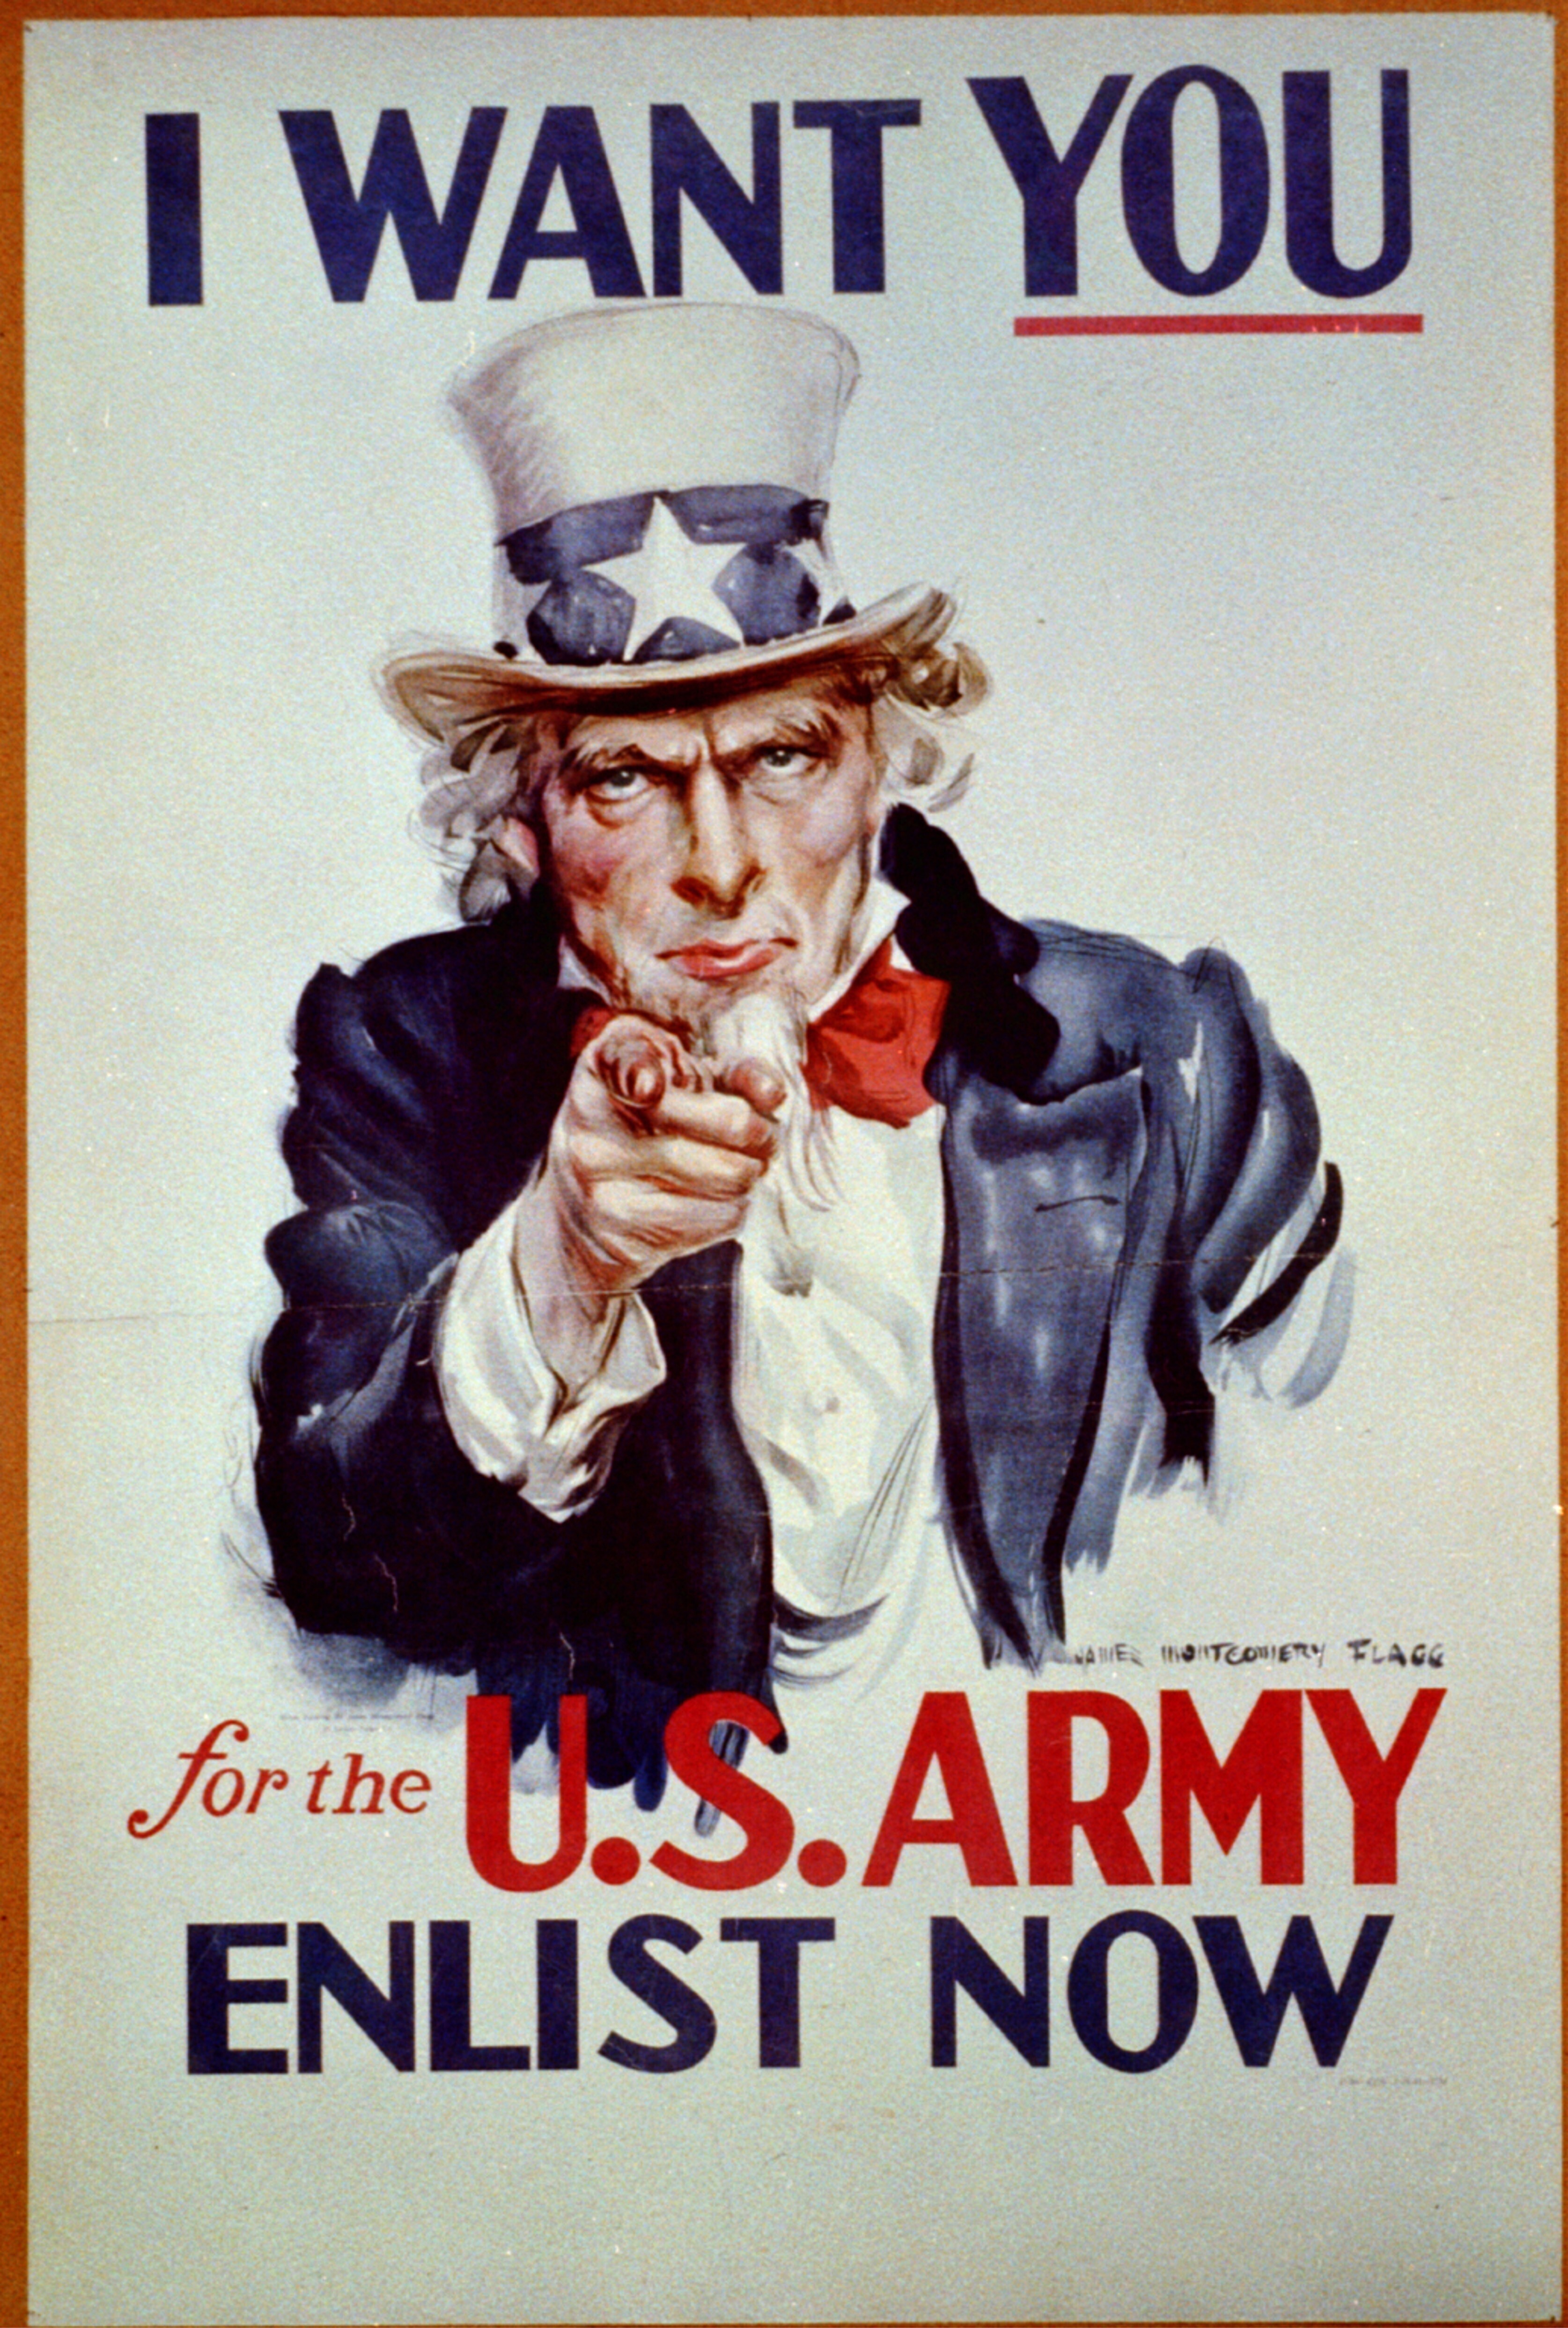
\includegraphics[keepaspectratio,width=.15\textwidth]{../../12_DataAnalysis/snapshot.jpg}
    \caption{注視画像}
    \label{fig:注視画像}
    \vspace{-1.5cm}
\end{wrapfigure}
\section{\method}
今回は,アイトラッキングするための装置としてTobii社の\tobi を用いる.注視する対象は\figref{fig:注視画像}で,
この実験の参加者は,学生の20代男性1名である.実験手続を以下に示す.
\begin{enumerate}
    \renewcommand{\labelenumi}{\fbox{\theenumi}}
    \item \tobi のメガネを装着する.
    \item 呈示されるマーカを追視し,視線方向のキャリブレーションを行う.
    \item 刺激(\figref{fig:注視画像})を自由に観察したときのGaze Plot,Heat Mapを作成する.
\end{enumerate}
\paragraph{Gaze PlotとHeat Map}
Gaze Plotは数値と円の大きさで,注視た順番と注視た時間を表現するグラフである.
数値は,注視した順番を表し,円の大きさは注視した時間を表す.円の大小と,注視時間は比例関係にある.
Heat Mapは注視時間が長い箇所を赤く表示する図である.

\begin{wrapfigure}{r}[0mm]{.42\textwidth}
    \vspace{-1cm}
    \centering
    \begin{minipage}[b]{.2\textwidth}
        \centering
        \includegraphics[keepaspectratio,width=\textwidth]{../../12_DataAnalysis/GazePlot.png}
        \subcaption{Gaze Plot}
    \end{minipage}
    \begin{minipage}[b]{.2\textwidth}
        \centering
        \includegraphics[keepaspectratio,width=\textwidth]{../../12_DataAnalysis/HeatMap.png}
        \subcaption{Heat Map}
    \end{minipage}
    \caption{\kadaid \ 実験結果}
    \label{fig:実験結果\kadaid}
    \vspace{-1.5cm}
\end{wrapfigure}
\section{\result}
作成したGaze PlotおよびHeat Mapを\figref{fig:実験結果\kadaid}に示す.
注視箇所について,差された指の指先と顔の中央,文字に集中していることが分かる.
注視した順番について,各番号の偏りは見られない.
\section{\consideration および\conclusion}
我々はポスターを見るときに,文字情報や被写体が印象に残る.
結果より,文字や被写体の顔部分をより多く注視しているからではないだろうか.
注視した順番については,全体的に偏りは見られないものの,文字列に対しては比較的小さい数値が出力されている.
我々は,まず文字から情報を得ようとするのではないだろうか.\par
この実験を通して,刺激画像の注視箇所と我々の印象に残っている点の因果を考察できた.
しかし,差された指の指先も注目すべき注視箇所だが,なぜ指先が多く注視されているのかの原因は分からなかった.